\chapter{Los iones y las disoluciones iónicas}\label{ch:g9:ions}

En un banco del gimnasio hay dos bebidas transparentes: una botella de
bebida isotónica, que se vende por sus ``electrolitos'', y un vaso de
agua con azúcar. En un laboratorio se sumergen por turnos en cada una
dos placas metálicas conectadas a una pila y a una bombilla pequeña. En
la bebida isotónica, la bombilla se enciende; en el agua con azúcar,
sigue apagada. Algo del primer líquido transporta carga eléctrica, y el
azúcar no. Ese algo son los \omterm{def:g9:ions:ion}{iones}.

\begin{recall}
Un \omterm{def:g7:atoms-and-molecules:atom}{átomo} tiene un \omterm{def:g9:inside-the-atom:nucleus}{núcleo} con $Z$ \omterm{def:g9:inside-the-atom:proton}{protones}, de carga $+e$ cada uno, y $Z$
\omterm{def:g9:inside-the-atom:nucleus}{electrones} a su alrededor, de carga $-e$ cada uno: el \omterm{def:g7:atoms-and-molecules:atom}{átomo} es neutro
(\cref{ch:g9:inside-the-atom}). Un \omterm{def:g6:solutions-and-solubility:solute}{soluto} disuelto en agua da una
\omterm{def:g6:solutions-and-solubility:solute}{disolución acuosa} (\cref{ch:g6:solutions-and-solubility}). Un \omterm{def:g7:identifying-substances:characteristic-test}{ensayo
característico} detecta una especie por un resultado visible
(\cref{ch:g7:identifying-substances}).
\end{recall}

\begin{omfigure}
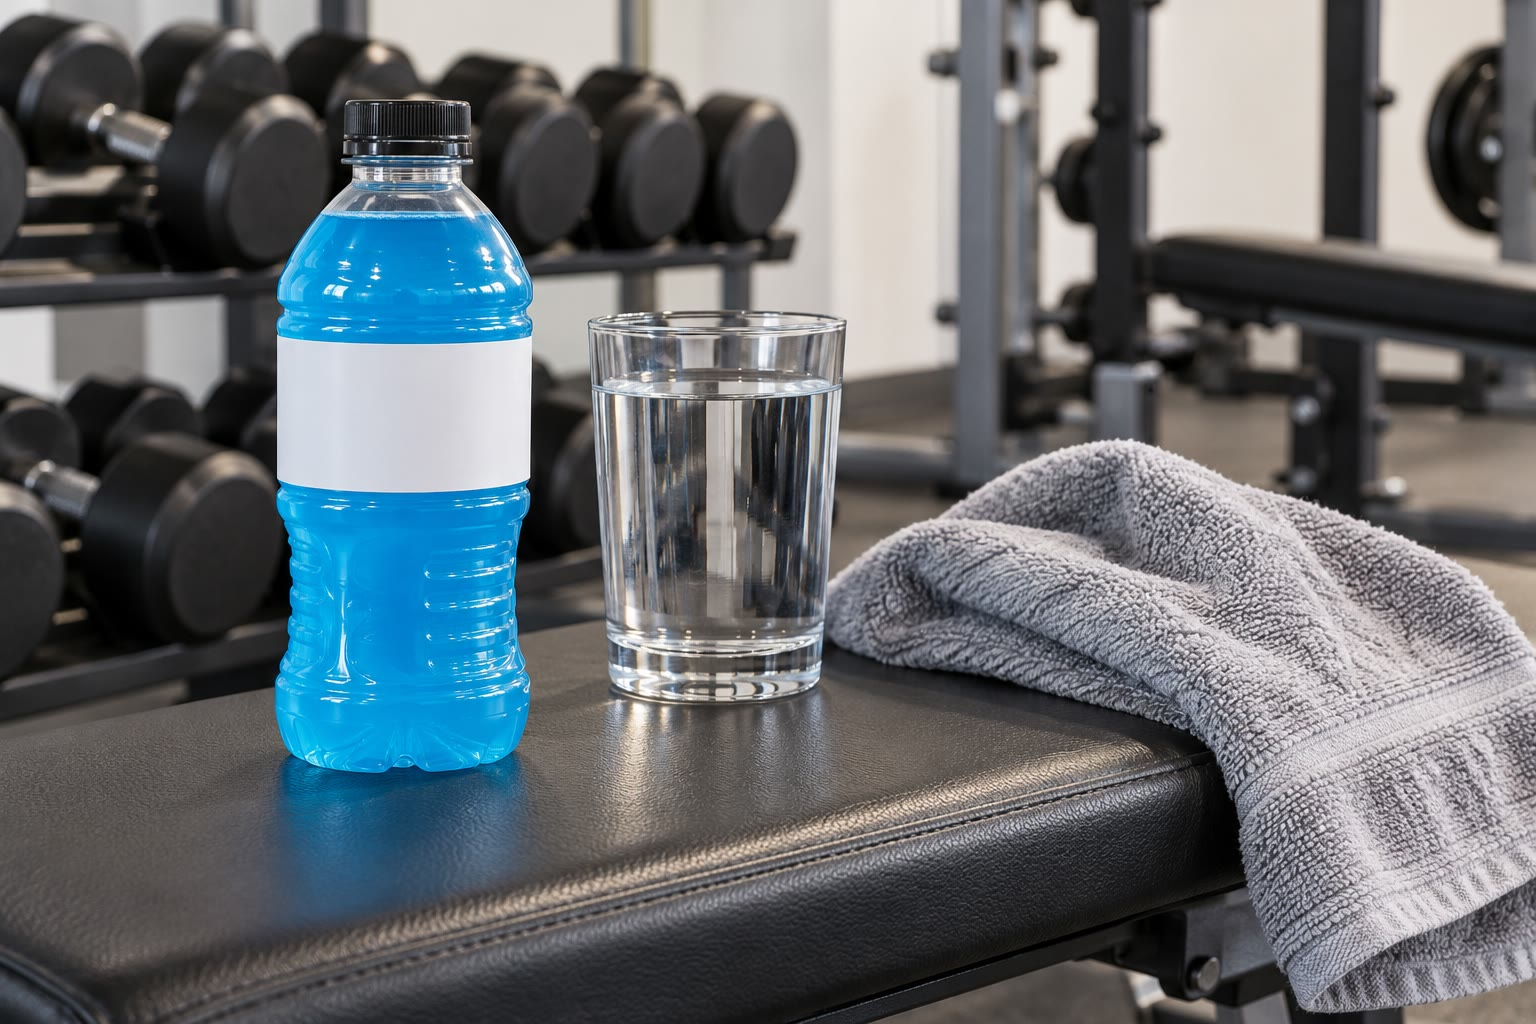
\includegraphics[width=0.5\linewidth]{images/book1/ai/g9-sports-drink.jpg}

{\small Una bebida isotónica y un vaso de agua: la bebida contiene \omterm{def:g9:ions:ion}{iones}
disueltos.}
\end{omfigure}

\section{Átomos que ganan o pierden electrones}

\begin{definition}[Ion, catión, anión]\label{def:g9:ions:ion}
Un \emph{ion}\index{ion} es un \omterm{def:g7:atoms-and-molecules:atom}{átomo}, o un grupo de \omterm{def:g7:atoms-and-molecules:atom}{átomos}, que ha
perdido o ganado uno o varios \omterm{def:g9:inside-the-atom:nucleus}{electrones}, y que por tanto tiene carga
eléctrica. Un ion con carga positiva, que ha perdido \omterm{def:g9:inside-the-atom:nucleus}{electrones}, es un
\emph{catión}\index{cation@catión}; un ion con carga negativa, que ha ganado
\omterm{def:g9:inside-the-atom:nucleus}{electrones}, es un \emph{anión}\index{anion@anión}. La carga se escribe arriba
a la derecha de la fórmula: \ce{Na+}, \ce{Cu^{2+}}, \ce{Cl-}.
\end{definition}

\begin{example}[El sodio y el cloro]\label{ex:g9:ions:na-cl}
Un \omterm{def:g7:atoms-and-molecules:atom}{átomo} de sodio, con 11 \omterm{def:g9:inside-the-atom:proton}{protones} y 11 \omterm{def:g9:inside-the-atom:nucleus}{electrones}, pierde un \omterm{def:g9:inside-the-atom:nucleus}{electrón}:
se convierte en el \omterm{def:g9:ions:ion}{ion} sodio \ce{Na+}, con 11 \omterm{def:g9:inside-the-atom:proton}{protones} y 10 \omterm{def:g9:inside-the-atom:nucleus}{electrones},
de carga
$+1$:
\[
  \ce{Na -> Na+ + e-}.
\]
Un \omterm{def:g7:atoms-and-molecules:atom}{átomo} de cloro, con 17 \omterm{def:g9:inside-the-atom:proton}{protones} y 17 \omterm{def:g9:inside-the-atom:nucleus}{electrones}, gana un \omterm{def:g9:inside-the-atom:nucleus}{electrón}:
se convierte en el \omterm{def:g9:ions:ion}{ion} cloruro \ce{Cl-}, con 17 \omterm{def:g9:inside-the-atom:proton}{protones} y 18
\omterm{def:g9:inside-the-atom:nucleus}{electrones}:
\[
  \ce{Cl + e- -> Cl-}.
\]
\end{example}

\begin{omfigure}
\begin{tikzpicture}[font=\small]
  \foreach \x/\name/\p/\e/\ch/\col in {0/{átomo de sodio}/11/11/0/omDef,
      3.7/{ion sodio \ce{Na+}}/11/10/+1/omProp,
      8.0/{átomo de cloro}/17/17/0/omDef, 11.7/{ion cloruro \ce{Cl-}}/17/18/$-1$/omProp} {
    \node[draw=\col, fill=\col!6, rounded corners=2pt, align=center, text width=2.4cm]
      at (\x,0) {\textbf{\name}\\ \p\ protones\\ \e\ electrones\\ carga \ch};
  }
  \draw[->, thick, omProp] (1.45,0) -- (2.25,0) node[midway, above, text=black,
    font=\footnotesize, align=center] {pierde\\ 1 \ce{e-}};
  \draw[->, thick, omProp] (9.45,0) -- (10.25,0) node[midway, above, text=black,
    font=\footnotesize, align=center] {gana\\ 1 \ce{e-}};
\end{tikzpicture}

{\small Un \omterm{def:g7:atoms-and-molecules:atom}{átomo} de sodio se convierte en un \omterm{def:g9:ions:ion}{ion} sodio al perder un
\omterm{def:g9:inside-the-atom:nucleus}{electrón}; un \omterm{def:g7:atoms-and-molecules:atom}{átomo} de cloro se convierte en un \omterm{def:g9:ions:ion}{ion} cloruro al ganar uno.
Los \omterm{def:g9:inside-the-atom:proton}{protones} no cambian.}
\end{omfigure}

\begin{proposition}[Algunos iones corrientes]\label{prop:g9:ions:common}
Los \omterm{def:g9:ions:ion}{iones} monoatómicos proceden de un solo \omterm{def:g7:atoms-and-molecules:atom}{átomo}; los poliatómicos, de
un grupo de \omterm{def:g7:atoms-and-molecules:atom}{átomos} que se mantiene unido:
\begin{center}
\small
\begin{tabular}{llll}
\hline
\omterm{def:g9:ions:ion}{cationes} & & \omterm{def:g9:ions:ion}{aniones} & \\
\hline
sodio & \ce{Na+} & cloruro & \ce{Cl-} \\
potasio & \ce{K+} & hidróxido & \ce{OH-} \\
calcio & \ce{Ca^{2+}} & nitrato & \ce{NO3-} \\
magnesio & \ce{Mg^{2+}} & carbonato & \ce{CO3^{2-}} \\
cobre(II) & \ce{Cu^{2+}} & sulfato & \ce{SO4^{2-}} \\
hierro(II), hierro(III) & \ce{Fe^{2+}}, \ce{Fe^{3+}} & & \\
cinc & \ce{Zn^{2+}} & & \\
aluminio & \ce{Al^{3+}} & & \\
amonio & \ce{NH4+} & & \\
\hline
\end{tabular}
\end{center}
\end{proposition}

\section{Los compuestos iónicos y sus fórmulas}

\begin{definition}[Compuesto iónico]\label{def:g9:ions:ionic-compound}
Un \emph{compuesto iónico}\index{compuesto ionico@compuesto iónico} está formado por
\omterm{def:g9:ions:ion}{cationes} y \omterm{def:g9:ions:ion}{aniones} en un número tal que el conjunto no tiene carga. Su
fórmula da la proporción de los \omterm{def:g9:ions:ion}{iones}, sin sus cargas: \ce{NaCl} para
el cloruro de sodio, un \ce{Na+} por cada \ce{Cl-}; \ce{CaCl2} para el
cloruro de calcio, dos \ce{Cl-} por cada \ce{Ca^{2+}}.
\end{definition}

\begin{method}[Escribir la fórmula de un compuesto iónico]\label{met:g9:ions:formula}
\begin{enumerate}
  \item Escribir los dos \omterm{def:g9:ions:ion}{iones} con sus cargas, el \omterm{def:g9:ions:ion}{catión} primero.
  \item Buscar los números más pequeños de cada uno que hacen nula la
        carga total.
  \item Escribir esos números como \omterm{def:g7:atoms-and-molecules:formula}{subíndices}; un \omterm{def:g9:ions:ion}{ion} poliatómico que
        necesita \omterm{def:g7:atoms-and-molecules:formula}{subíndice} va entre paréntesis.
\end{enumerate}
Óxido de aluminio: \ce{Al^{3+}} y \ce{O^{2-}}; $2 \times (+3) + 3 \times
(-2) = 0$, así que \ce{Al2O3}. Hidróxido de hierro(III): \ce{Fe^{3+}} y
tres
\ce{OH-}: \ce{Fe(OH)3}.
\end{method}

\begin{proposition}[Un sólido iónico es un apilamiento de iones]\label{prop:g9:ions:solid}
En un cristal de sal, los \omterm{def:g9:ions:ion}{iones} sodio y los \omterm{def:g9:ions:ion}{iones} cloruro se alternan en
un apilamiento regular en tres dimensiones, y cada \omterm{def:g9:ions:ion}{ion} está rodeado de
\omterm{def:g9:ions:ion}{iones} de carga opuesta, que lo mantienen en su sitio. Un grano de sal de
mesa contiene trillones de ellos; su forma cúbica refleja el
apilamiento cúbico.
\end{proposition}

\begin{omfigure}
\begin{minipage}[b]{0.5\linewidth}\centering
\begin{tikzpicture}[font=\small]
  \foreach \i in {0,...,5} \foreach \j in {0,...,4} {
    \pgfmathtruncatemacro\pp{mod(\i+\j,2)}
    \ifnum\pp=0 \node[aNa, minimum size=5mm] at (0.62*\i,0.62*\j) {};
    \else \node[aCl, minimum size=7.4mm] at (0.62*\i,0.62*\j) {};\fi
  }
\end{tikzpicture}

{\small Una capa de un cristal de sal: los \omterm{def:g9:ions:ion}{iones} sodio (morados, más
pequeños) y los \omterm{def:g9:ions:ion}{iones} cloruro (verdes) se alternan.}
\end{minipage}\hfill
\begin{minipage}[b]{0.3\linewidth}\centering
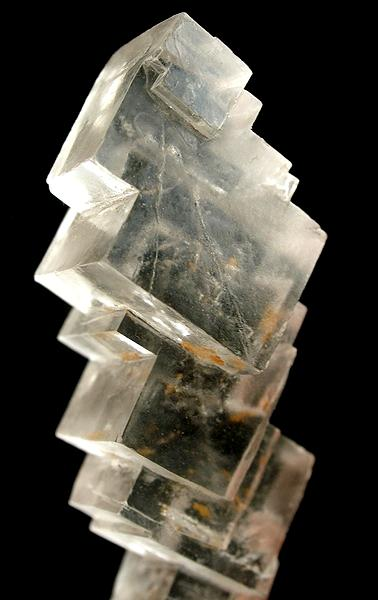
\includegraphics[height=4.6cm]{images/book1/halite.jpg}

{\small Halita, la sal gema natural. Foto: Robert M.~Lavinsky,
CC BY-SA 3.0.}
\end{minipage}
\end{omfigure}

\section{Las disoluciones iónicas conducen la electricidad}

\begin{notation}[El símbolo de estado (aq)]\label{not:g9:ions:aq}
Un \omterm{def:g9:ions:ion}{ion} o una \omterm{def:g7:atoms-and-molecules:molecule}{molécula} disueltos en agua se marcan con (aq), de
``acuoso'':
\ce{Na+(aq)}, \ce{Cl-(aq)}.
\end{notation}

\begin{proposition}[Las disoluciones iónicas conducen la electricidad]\label{prop:g9:ions:conduct}
Cuando un \omterm{def:g9:ions:ionic-compound}{compuesto iónico} se \omterm{def:g2:mixing-and-dissolving:dissolve}{disuelve} en agua, sus \omterm{def:g9:ions:ion}{iones} se separan y
se mueven libremente por la disolución: el agua salada contiene
\ce{Na+(aq)} y \ce{Cl-(aq)}. Los \omterm{def:g9:ions:ion}{iones} en movimiento transportan carga
eléctrica, así que una disolución iónica conduce la electricidad. Una
disolución de azúcar, cuyas \omterm{def:g7:atoms-and-molecules:molecule}{moléculas} no tienen carga, no la conduce; el
agua muy pura, tampoco.
\end{proposition}

\begin{inthelab}[¿Qué líquidos conducen?]
El profesor monta un circuito con dos placas metálicas, una pila de
bajo voltaje y una bombilla pequeña; sumerge las placas por turnos en
agua destilada, agua con azúcar, agua salada y una disolución de sulfato
de cobre, y las enjuaga entre una y otra. La bombilla solo se enciende
con las dos disoluciones iónicas.
\end{inthelab}

\begin{omfigure}
\begin{tikzpicture}[font=\small, scale=1.1]
  \foreach \xs/\lit/\lab in {0/1/{agua salada: se enciende}, 5.2/0/{agua con azúcar: apagada}} {
    \begin{scope}[xshift=\xs cm]
      \pic[transform shape] at (2,0) {beaker={0.7}{omWater!80}};
      \fill[black!45] (1.6,0.25) rectangle (1.7,2.6);
      \fill[black!45] (2.3,0.25) rectangle (2.4,2.6);
      \ifnum\lit=1 \fill[yellow!70, opacity=0.8] (3.4,3.0) circle (0.42);\fi
      \draw (1.65,2.6) -- (1.65,3.6) to[battery1] (3.4,3.6) -- (3.4,3.4)
        to[lamp] (3.4,2.6) -- (2.35,2.6);
      \node[anchor=north, align=center] at (2,-0.15) {\lab};
    \end{scope}
  }
\end{tikzpicture}

{\small El ensayo de conductividad: con agua salada, los \omterm{def:g9:ions:ion}{iones}
transportan la corriente y la bombilla se enciende; el agua con azúcar
no contiene \omterm{def:g9:ions:ion}{iones} y la bombilla sigue apagada.}
\end{omfigure}

\section{Ensayos de precipitación de iones}

\begin{definition}[Precipitado]\label{def:g9:ions:precipitate}
Cuando se \omterm{def:g2:mixing-and-dissolving:mix}{mezclan} dos disoluciones, un \omterm{def:g9:ions:ion}{catión} de una y un \omterm{def:g9:ions:ion}{anión} de la
otra pueden formar un \omterm{def:g9:ions:ionic-compound}{compuesto iónico} que no se \omterm{def:g2:mixing-and-dissolving:dissolve}{disuelve}. Aparece como
un sólido fino que enturbia el líquido y se deposita: un
\emph{precipitado}\index{precipitado}. La reacción es una
\emph{precipitación}\index{precipitacion@precipitación}.
\end{definition}

\begin{proposition}[Ensayos de iones corrientes]\label{prop:g9:ions:tests}
Unas gotas de una disolución de \omterm{def:g7:chemical-reactions:reactant}{reactivo} identifican un \omterm{def:g9:ions:ion}{ion} por el color
del \omterm{def:g9:ions:precipitate}{precipitado} que forma:
\begin{center}
\small
\begin{tabular}{llll}
\hline
\omterm{def:g9:ions:ion}{ion} buscado & \omterm{def:g7:chemical-reactions:reactant}{reactivo} & \omterm{def:g9:ions:precipitate}{precipitado} & color \\
\hline
cobre(II) \ce{Cu^{2+}} & hidróxido de sodio & \ce{Cu(OH)2} & azul \\
hierro(II) \ce{Fe^{2+}} & hidróxido de sodio & \ce{Fe(OH)2} & verde \\
hierro(III) \ce{Fe^{3+}} & hidróxido de sodio & \ce{Fe(OH)3} & pardo anaranjado \\
cinc \ce{Zn^{2+}} & hidróxido de sodio & \ce{Zn(OH)2} & blanco \\
aluminio \ce{Al^{3+}} & hidróxido de sodio & \ce{Al(OH)3} & blanco \\
cloruro \ce{Cl-} & nitrato de plata & \ce{AgCl} & blanco, se oscurece a la luz \\
\hline
\end{tabular}
\end{center}
\end{proposition}

\begin{example}[Escribir una precipitación]\label{ex:g9:ions:equation}
Solo se escriben los \omterm{def:g9:ions:ion}{iones} que forman el sólido; los demás siguen
disueltos y no intervienen:
\[
  \ce{Cu^{2+}(aq) + 2OH-(aq) -> Cu(OH)2(s)}, \qquad
  \ce{Ag+(aq) + Cl-(aq) -> AgCl(s)}.
\]
\end{example}

\begin{omfigure}
\begin{tikzpicture}[font=\small, scale=0.95]
  \foreach \k/\pc/\lab in {0/blue!60/{\ce{Cu^{2+}}: azul}, 1/green!45!black!70/{\ce{Fe^{2+}}: verde},
      2/orange!70!brown/{\ce{Fe^{3+}}: pardo\\anaranjado}, 3/white!85!black/{\ce{Zn^{2+}}: blanco},
      4/white!85!black/{\ce{Al^{3+}}: blanco}, 5/white!80!black/{\ce{Cl-}: blanco}} {
    \pic[transform shape] at (\k*2.3,0) {testtube={0.5}{omWater!60}};
    \pic[transform shape] at (\k*2.3,0) {testtube={0.14}{\pc}};
    \node[anchor=north, align=center, font=\footnotesize, text width=2cm] at (\k*2.3,-0.15) {\lab};
  }
\end{tikzpicture}

{\small \omterm{def:g9:ions:precipitate}{Precipitados} formados con hidróxido de sodio (los cinco primeros
tubos) y con nitrato de plata (el último tubo).}
\end{omfigure}

\begin{safety}{\ghs[0.82cm]{GHS05}\ghs[0.82cm]{GHS07}}
% ledger: ghs:NaOH, ghs:AgNO3
Hidróxido de sodio: provoca quemaduras graves en la piel y lesiones
oculares graves, y puede ser corrosivo para los metales (GHS05); diluido,
irrita la piel y los ojos (GHS07). El nitrato de plata, el \omterm{def:g7:chemical-reactions:reactant}{reactivo} del
cloruro, es comburente, corrosivo y muy tóxico para los organismos
acuáticos. Gafas y guantes; el profesor reparte los \omterm{def:g7:chemical-reactions:reactant}{reactivos} gota a
gota.
\end{safety}

\begin{method}[Ensayar un ion]\label{met:g9:ions:test}
\begin{enumerate}
  \item Verter un poco de la disolución que se quiere ensayar en un tubo
        de ensayo.
  \item Añadir el \omterm{def:g7:chemical-reactions:reactant}{reactivo} gota a gota.
  \item Anotar el color de un posible \omterm{def:g9:ions:precipitate}{precipitado} y compararlo con la
        tabla.
  \item Concluir, recordando que un ensayo identifica un \omterm{def:g9:ions:ion}{ion}, no un
        compuesto: la disolución de cloruro de hierro(III) da positivo
        tanto en el ensayo del \ce{Fe^{3+}} como en el del \ce{Cl-}.
\end{enumerate}
\end{method}

\section{Ejercicios}

\begin{exercise}[$\star$]\label{exo:g9:ions:1}
¿Qué es un \omterm{def:g9:ions:ion}{ion}? ¿Qué diferencia hay entre un \omterm{def:g9:ions:ion}{catión} y un \omterm{def:g9:ions:ion}{anión}?
\end{exercise}

\begin{exercise}[$\star$]\label{exo:g9:ions:2}
Un \omterm{def:g7:atoms-and-molecules:atom}{átomo} de magnesio (12 \omterm{def:g9:inside-the-atom:proton}{protones}) pierde dos \omterm{def:g9:inside-the-atom:nucleus}{electrones}. Escribe la
fórmula del \omterm{def:g9:ions:ion}{ion} formado y da su número de \omterm{def:g9:inside-the-atom:proton}{protones} y de \omterm{def:g9:inside-the-atom:nucleus}{electrones}.
\end{exercise}

\begin{exercise}[$\star$]\label{exo:g9:ions:3}
Escribe las fórmulas del cloruro de potasio, el cloruro de magnesio y el
óxido de calcio (\omterm{def:g9:ions:ion}{ion} óxido: \ce{O^{2-}}).
\end{exercise}

\begin{exercise}[$\star$]\label{exo:g9:ions:4}
¿Por qué el agua salada conduce la electricidad y el agua con azúcar no?
\end{exercise}

\begin{exercise}[$\star\star$]\label{exo:g9:ions:5}
Escribe las fórmulas del sulfato de cobre(II), el cloruro de aluminio y
el carbonato de sodio.
\end{exercise}

\begin{exercise}[$\star\star$]\label{exo:g9:ions:6}
Al añadir hidróxido de sodio a una disolución se forma un \omterm{def:g9:ions:precipitate}{precipitado}
pardo anaranjado. ¿Qué \omterm{def:g9:ions:ion}{ion} contiene la disolución? Escribe la ecuación
de la \omterm{def:g9:ions:precipitate}{precipitación}.
\end{exercise}

\begin{exercise}[$\star\star$]\label{exo:g9:ions:7}
¿Cuántos \omterm{def:g9:inside-the-atom:nucleus}{electrones} tiene el \omterm{def:g9:ions:ion}{ion} sulfato \ce{SO4^{2-}} de más respecto a
sus \omterm{def:g9:inside-the-atom:proton}{protones}? ¿Y el \omterm{def:g9:ions:ion}{ion} nitrato \ce{NO3-}?
\end{exercise}

\begin{exercise}[$\star\star$]\label{exo:g9:ions:8}
Una disolución da un \omterm{def:g9:ions:precipitate}{precipitado} blanco con nitrato de plata y uno azul
con hidróxido de sodio. Nombra el \omterm{def:g9:ions:ionic-compound}{compuesto iónico} disuelto y escribe
su fórmula.
\end{exercise}

\begin{exercise}[$\star\star$]\label{exo:g9:ions:9}
Mira la figura de la capa del cristal de sal. ¿Cuántos vecinos de carga
opuesta tiene, en esa capa, un \omterm{def:g9:ions:ion}{ion} situado en el centro?
\end{exercise}

\begin{exercise}[$\star\star$]\label{exo:g9:ions:10}
Escribe la ecuación de la \omterm{def:g9:ions:precipitate}{precipitación} del hidróxido de hierro(II) a
partir de los \omterm{def:g9:ions:ion}{iones} \ce{Fe^{2+}} y \ce{OH-}.
\end{exercise}

\begin{exercise}[$\star\star\star$]\label{exo:g9:ions:11}
Un polvo blanco puede ser cloruro de cinc o cloruro de sodio. Disuelto en
agua, da un \omterm{def:g9:ions:precipitate}{precipitado} blanco con hidróxido de sodio. ¿Cuál es?
Escribe la ecuación.
\end{exercise}

\begin{exercise}[$\star\star\star$]\label{exo:g9:ions:12}
En un cristal de cloruro de calcio, ¿cuántos \omterm{def:g9:ions:ion}{iones} cloruro hay por cada
1000 \omterm{def:g9:ions:ion}{iones} calcio? Comprueba que el cristal es neutro.
\end{exercise}

\section{Problema: El pozo oxidado}

\begin{problem}[{Problema de fin de semana --- manchas anaranjadas en el
fregadero de una granja, dos ensayos y el número de iones hierro en un
litro de agua de pozo}]
\label{pb:g9:ions:1}
El agua del pozo de una granja deja manchas anaranjadas en el
fregadero. Un laboratorio recibe una muestra. Recién sacada, el agua es
transparente; con hidróxido de sodio da un \omterm{def:g9:ions:precipitate}{precipitado} verde, que en
menos de una hora se vuelve pardo anaranjado en la superficie, donde
está en contacto con el \omterm{def:g4:air-a-mixture-of-gases:air}{aire}. El laboratorio mide \qty{0.30}{mg} de
hierro, en forma de \omterm{def:g9:ions:ion}{iones} hierro, por litro. Toma como masa de un
\omterm{def:g9:inside-the-atom:proton}{nucleón} \qty{1.67e-27}{kg}, y 56 \omterm{def:g9:inside-the-atom:proton}{nucleones} para un \omterm{def:g7:atoms-and-molecules:atom}{átomo} de hierro.

\medskip
\noindent\textbf{Parte I --- Los ensayos.}
\begin{enumerate}
  \item ¿Qué \omterm{def:g9:ions:ion}{ion} muestra el \omterm{def:g9:ions:precipitate}{precipitado} verde? Da la fórmula del
        \omterm{def:g9:ions:precipitate}{precipitado}.
  \item ¿Qué \omterm{def:g9:ions:ion}{ion} muestra el \omterm{def:g9:ions:precipitate}{precipitado} pardo anaranjado? Da su
        fórmula.
  \item Un \omterm{def:g9:ions:ion}{ion} hierro(II) y un \omterm{def:g9:ions:ion}{ion} hierro(III) se diferencian en un
        \omterm{def:g9:inside-the-atom:nucleus}{electrón}. ¿Cuál tiene más \omterm{def:g9:inside-the-atom:nucleus}{electrones}? ¿Cuántos \omterm{def:g9:inside-the-atom:nucleus}{electrones} tiene
        cada uno (hierro: $Z = 26$)?
  \item Escribe la ecuación de la \omterm{def:g9:ions:precipitate}{precipitación} del hidróxido de
        hierro(III).
\end{enumerate}

\medskip
\noindent\textbf{Parte II --- Las manchas.}
\begin{enumerate}[resume]
  \item En el fregadero, el agua transparente se va enturbiando y
        volviendo anaranjada. ¿Qué \omterm{def:g9:ions:ion}{ion} contiene el agua cuando sale del
        pozo, y cuál acaba conteniendo?
  \item Escribe la fórmula del \omterm{def:g9:ions:ionic-compound}{compuesto iónico} formado por los \omterm{def:g9:ions:ion}{iones}
        hierro(III) y los \omterm{def:g9:ions:ion}{iones} hidróxido, y comprueba que es neutro.
  \item ¿Se puede eliminar el hierro del agua filtrándola en cuanto sale
        del pozo? ¿Y después de que se haya vuelto anaranjada?
        Explícalo.
  \item ¿Un agua que contiene \omterm{def:g9:ions:ion}{iones} hierro es una \omterm{def:g6:pure-substances-and-mixtures:pure-substance}{sustancia pura}? ¿Una
        \omterm{def:g6:pure-substances-and-mixtures:homogeneous}{mezcla homogénea}?
\end{enumerate}

\medskip
\noindent\textbf{Parte III --- Contar los \omterm{def:g9:ions:ion}{iones}.}
\begin{enumerate}[resume]
  \item Calcula la masa de un \omterm{def:g7:atoms-and-molecules:atom}{átomo} de hierro, en kilogramos.
  \item Convierte \qty{0.30}{mg} en kilogramos.
  \item ¿Por qué se puede tomar la masa de un \omterm{def:g9:ions:ion}{ion} hierro igual a la de un
        \omterm{def:g7:atoms-and-molecules:atom}{átomo} de hierro?
  \item Calcula el número de \omterm{def:g9:ions:ion}{iones} hierro que hay en un litro del agua
        del pozo.
\end{enumerate}
\end{problem}
